\documentclass[a4paper,conference]{IEEEtran}
\IEEEoverridecommandlockouts
% IDAP'26 LaTeX template adapted from the conference-provided file.

\usepackage[utf8]{inputenc}
\usepackage[T1]{fontenc}
\usepackage[english]{babel}
\usepackage{cite}
\usepackage{amsmath,amssymb,amsfonts}
\usepackage{graphicx}
\usepackage{textcomp}
\usepackage{xcolor}
\usepackage{booktabs}
\usepackage{array}
\usepackage{tabularx}
\usepackage{multirow}
\usepackage{url}
\usepackage{fancyhdr}

\newcolumntype{Y}{>{\raggedright\arraybackslash}X}
\newcolumntype{C}{>{\centering\arraybackslash}X}
\renewcommand{\arraystretch}{1.10}
\urlstyle{same}

\fancypagestyle{firstpage}{%
  \fancyhf{}%
  \fancyhead[L]{\footnotesize 10th International Artificial Intelligence and Data Processing Symposium (IDAP'26), Sept 5--6, 2026, Türkiye (Malatya--İstanbul), Philippines}
  \renewcommand{\headrulewidth}{0pt}%
}

\begin{document}

\title{SACI: Explainable Graph-Supported Scoring of Scope-Bounded SIEM-CTI Evidence Coverage}

\author{\IEEEauthorblockN{İsmet Arslan}
\IEEEauthorblockA{\textit{Department of Computer Engineering} \\
\textit{Karamanoğlu Mehmetbey University}\\
Karaman, Türkiye \\
\texttt{https://v4gus.com} \\ \texttt{https://github.com/4rslanismet}}}

\maketitle
\thispagestyle{firstpage}

\begin{abstract}
Security information and event management platforms aggregate heterogeneous telemetry, yet platform deployment alone does not establish whether critical assets, expected sources, detection controls, ATT\&CK mappings, and cyber-threat-intelligence workflows are observably connected. This paper presents SACI, a deterministic protocol for measuring scope-bounded SIEM--CTI evidence coverage with graph provenance and fail-closed publication validation. Five normalized components are combined through an explicit simple additive weighting design with active-weight renormalization. In a controlled six-asset Wazuh--MISP laboratory, the canonical snapshot closed 12/12 expected asset--source pairs, 25/25 enabled controls, 13/13 in-scope ATT\&CK techniques, and 8/8 configured CTI workflow flags, yielding a component vector and SACI score of 100. A pre-release inconsistency case showed that complete relationship-row closure can coexist with an invalid graph representation. The resulting integrity gate was therefore evaluated with nine controlled structural cases covering undeclared endpoints, duplicate identifiers, mapping conflicts, representation mismatch, missing fields, parallel-evidence identity, and isolation policy; all cases produced their preregistered status. A synthetic cardinality benchmark replicated the canonical 99-node/171-row structure up to 99,000 nodes and 171,000 edge rows; the single-process Python validator completed the largest case in a median 0.88~s with 41.17~MiB peak traced memory. A separate twenty-condition sensitivity suite produced directionally expected score changes. SACI is thus positioned as an auditable measurement and publication-control protocol for a declared evidence universe.
\end{abstract}

\begin{IEEEkeywords}
SIEM, Wazuh, cyber threat intelligence, MITRE ATT\&CK, evidence graph, security measurement, explainability, reproducibility, integrity validation
\end{IEEEkeywords}

\section{Introduction}
Security operations centers depend on heterogeneous endpoint, identity, network, application, and threat-intelligence telemetry. Log-management guidance emphasizes collecting, transporting, retaining, and analyzing security-relevant records, while continuous-monitoring guidance requires evidence to be interpreted over time and within organizational context \cite{nist80092,nist800137,nistcsf20}. Nevertheless, a deployed SIEM does not by itself establish that every critical asset emits the expected sources, that enabled detection controls have produced observable evidence, or that ATT\&CK mappings correspond to actually monitored data.

This distinction matters because operational visibility can fail without an obvious platform outage. A high alert volume may coexist with a silent critical source, a stale endpoint, an enabled rule that never fires, a technique identifier copied from a configuration file but unsupported by live evidence, or an IOC lookup that is expected but not demonstrably executed. ATT\&CK provides a shared language for adversary behavior and data sources, yet both MITRE and CISA stress the importance of accurate mapping and evidence-aware interpretation \cite{mitre_matrix,mitre_datasources,mitre_philosophy,cisa_mapping}. The open-world difficulty is fundamental: absence of an observed relation may indicate true absence, missing collection, an attribution error, or an incomplete dataset \cite{sommer2010}.

Existing attack-surface metrics quantify exposed resources or compare system versions \cite{manadhata2011}. ATT\&CK rating approaches summarize technical coverage \cite{manocha2021,alsada2023}, CTI platforms organize and exchange indicators and contextual objects \cite{wagner2016,mavroeidis2017,oasis_stix,oasis_taxii}, and cybersecurity knowledge graphs join heterogeneous entities for provenance and analysis \cite{liu2022,w3cprov}. These contributions are valuable, but they do not directly answer a narrower operational question: within a declared SIEM-CTI evidence universe, which expected relationships are actually closed, how does each closure contribute to a deterministic score, and can the published dataset be rejected when its graph structure is invalid even though the score is numerically complete?

This paper presents SACI as a scope-bounded evidence-coverage index. The graph supports provenance, integrity, and explanation; it does not replace the coverage formulas or convert the result into a graph-theoretic risk probability. SACI is therefore \emph{graph-supported}, not graph-derived. The model deliberately separates four concepts: (i) declared evaluation scope, (ii) observed evidence, (iii) numerical coverage, and (iv) publication integrity.

The study addresses four research questions:
\begin{itemize}
    \item \textbf{RQ1:} Can heterogeneous SIEM telemetry, ATT\&CK mappings, controls, and CTI workflow evidence be transformed into an auditable, scope-bounded coverage score?
    \item \textbf{RQ2:} Can an independent integrity gate distinguish numerically closed evidence from structurally invalid publication artifacts?
    \item \textbf{RQ3:} Does the score respond in the intended direction to controlled telemetry, control, CTI, and freshness perturbations?
    \item \textbf{RQ4:} How does integrity validation behave under controlled structural faults and synthetic increases in graph cardinality?
\end{itemize}

The contributions are sixfold. First, the paper defines a typed provenance graph that connects assets, log sources, controls, Wazuh rules, ATT\&CK techniques, IOC objects, platforms, integrations, metrics, and reason codes. Second, it operationalizes five auditable security-measurement components through transparent ratios and simple additive weighting with active-weight normalization \cite{nist80055v1,nist80055v2,iso27004,triantaphyllou2000}; the contribution is the evidence semantics and audit protocol rather than a new aggregation operator. Third, it introduces a fail-closed integrity gate that distinguishes edge closure from endpoint validity, mapping consistency, representation consistency, parallel-evidence identity, and isolation policy. Fourth, it validates that gate through a pre-release inconsistency case and nine controlled structural fault cases. Fifth, it evaluates coverage behavior in a controlled six-asset Wazuh--MISP laboratory, a twenty-condition score-sensitivity suite, and a synthetic integrity-cardinality benchmark. Sixth, it publishes a machine-readable research companion with source code, CSV/JSON/CYJS artifacts, benchmark outputs, SHA-256 records, validators, and a Vagrant-based reproduction scaffold \cite{fips1804,vagrant_docs,github_pages,github_actions,arslan_artifact}.

\begin{figure*}[!t]
\centering
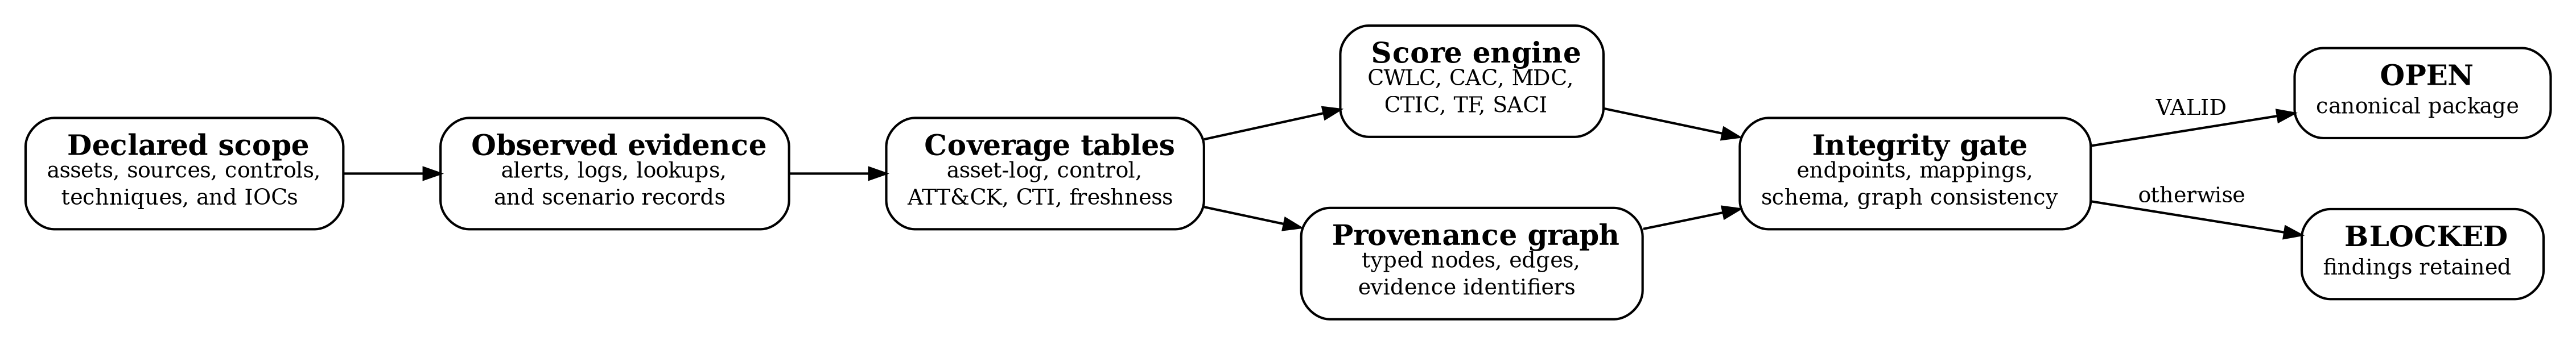
\includegraphics[width=0.96\textwidth]{figures/saci_pipeline.png}
\caption{SACI evidence-processing, scoring, graph-provenance, and fail-closed publication pipeline.}
\label{fig:pipeline}
\end{figure*}

\section{Related Work}
\subsection{Security Measurement, Log Management, and Attack Surface}
NIST SP 800-55 recommends defining security measures with their purpose, scope, data, calculation, interpretation, and decision use; Volume 2 extends this into a measurement program \cite{nist80055v1,nist80055v2}. ISO/IEC 27004 similarly frames monitoring, measurement, analysis, and evaluation as management-system activities \cite{iso27004}. SACI follows this measurement discipline by fixing denominators before observing outcomes, publishing numerators and denominators separately, and treating weights as explicit design parameters rather than probabilities.

The composite uses the simple additive weighting form commonly discussed in multi-criteria decision analysis \cite{triantaphyllou2000}. Its use here is intentionally conservative: all components are normalized to a common 0--100 scale, monotonicity is explicit, and the component vector remains visible beside the aggregate. SACI therefore does not claim a new multi-criteria operator; it contributes domain-specific evidence units, applicability rules, provenance, and publication validation.

NIST SP 800-92 provides enterprise log-management guidance, while SP 800-137 treats continuous monitoring as a repeated evidence process rather than a one-time configuration check \cite{nist80092,nist800137}. SACI operationalizes these ideas at the asset-log-source and enabled-control levels. In contrast, the attack-surface metric of Manadhata and Wing estimates relative exposure through a system's resources and attackability \cite{manadhata2011}. SACI does not estimate exposure magnitude or compromise likelihood. It measures the closure of declared monitoring and enrichment relationships and should therefore not be interpreted as a replacement for classical attack-surface or risk metrics.

\subsection{ATT\&CK Coverage and Detection Engineering}
ATT\&CK is a knowledge base of adversary tactics and techniques derived from real-world observations \cite{mitre_matrix,mitre_philosophy}. Its data-source model identifies subjects and data components that may support detection \cite{mitre_datasources}. CISA's mapping guide warns that behavior should be mapped at the appropriate level of specificity and with defensible evidence \cite{cisa_mapping}. Wazuh can attach ATT\&CK metadata to rules and alerts \cite{wazuh_mitre}, while tools such as DeTT\&CT organize visibility and detection mappings across techniques \cite{dettect}. D3FEND provides a complementary knowledge graph for defensive techniques \cite{d3fend}.

ATT\&CK-based rating frameworks demonstrate the usefulness of summary coverage measures, but technique counts alone can hide whether a mapped rule is enabled, whether the necessary source is present, and whether the rule produced evidence \cite{manocha2021,alsada2023}. SACI therefore constrains MDC to a declared technique subset and links technique closure to rules, controls, and source provenance. It also separates direct rule mapping from contextual CTI association so that an enrichment result does not silently become native detection logic.

\subsection{Cyber Threat Intelligence and Typed Evidence Graphs}
STIX 2.1 specifies machine-readable cyber-threat objects and relationships, while TAXII 2.1 defines an application-layer exchange protocol \cite{oasis_stix,oasis_taxii}. MISP implements collaborative storage, sharing, and operational use of threat information \cite{wagner2016,misp_docs}; its taxonomy and scoring mechanisms also illustrate that indicator context and freshness require explicit policy \cite{mokaddem2019}. CTI taxonomies and ontologies improve interoperability, but external context still has to be bound to internal observations \cite{mavroeidis2017}.

Knowledge graphs can unify multi-source cybersecurity entities, events, vulnerabilities, and intelligence objects \cite{liu2022}. W3C PROV-O provides a general vocabulary for representing provenance among entities, activities, and agents \cite{w3cprov}. Constraint languages such as SHACL formalize graph-shape validation, while work such as Trav-SHACL studies efficient validation over large constraint networks \cite{w3c_shacl,figuera2021travshacl}. SACI follows the same general principle that a graph should be validated against explicit structural expectations, but it does not implement an RDF/SHACL engine. Its publication artifacts are CSV and property-graph representations checked by a purpose-built validator. Every canonical relationship row has a typed source, a typed target, an observation state, and a stable evidence identifier. Cytoscape.js and Mermaid provide interactive and text-defined representations of the same graph \cite{cytoscapejs,mermaid}; neither representation is treated as an independent ground truth.

\subsection{Reproducibility and Explanation}
Reproducibility requires distinguishing repeatability of a computational artifact from independent reconstruction of an entire environment \cite{nas_repro,acm_artifacts}. Vagrant can express machine roles and provisioning entry points, while provider-specific behavior remains dependent on boxes, plugins, networks, and credentials \cite{vagrant_docs,vagrant_vmware}. GitHub Pages supports a static research companion and GitHub Actions can automate validation workflows \cite{github_pages,github_actions}. SACI therefore reports artifact reproducibility and environment reproducibility as different assurance levels.

The explanation layer is also separated from calculation. Deterministic reason codes explain score gaps. A local language model may summarize only validated artifacts through retrieval-augmented generation \cite{lewis2020}, subject to governance and traceability principles in the NIST AI RMF and its generative-AI profile \cite{nist_airmf,nist_genai}. No language model computes or changes the numerical score or integrity status in this study.

\section{SACI Method}
\subsection{Scope and Typed Graph}
Let the evidence graph be $G=(V,E)$. The node set $V$ is the union of assets, log sources, detection controls, Wazuh rules, ATT\&CK techniques, IOC objects, platforms, integrations, score metrics, and reason codes. The directed edge set $E$ uses typed relations including \texttt{emits}, \texttt{collected\_by}, \texttt{protected\_by}, \texttt{uses\_log\_source}, \texttt{produces\_rule}, \texttt{alerted\_in}, \texttt{detects\_technique}, \texttt{contains\_ioc}, \texttt{queries}, \texttt{matches\_ioc}, \texttt{converted\_to\_alert}, \texttt{mapped\_to}, \texttt{contextualized\_as}, \texttt{contributes\_to}, \texttt{triggers\_integration}, \texttt{contains}, \texttt{uses}, and \texttt{maps\_to}.

An edge row carries at least $(source, relationship, target, observed)$. In the canonical release it additionally carries \texttt{evidence\_id}, \texttt{evidence\_origin}, and where relevant \texttt{mapping\_basis}. The score is calculated from normalized coverage tables. The graph is derived from those tables to preserve provenance and to expose structural defects; it is not a second measurement dataset.

\subsection{Operational Metric Design}
Table~\ref{tab:metrics} summarizes the five components. All component scores lie in $[0,100]$. A metric that is genuinely not applicable is removed from both numerator and denominator of the composite score. Missing required evidence, a failed query, or a malformed file is not silently converted to N/A; it is reported as an evidence gap or an incomplete run.

The composite in (\ref{eq:saci}) is a simple additive weighting operationalization \cite{triantaphyllou2000}. This choice favors traceability over mathematical novelty: a reviewer can reproduce every component, inspect the declared weights, and compare the aggregate with the full vector. The fixed study weights express prioritization within this laboratory and are not presented as statistically learned or universally optimal parameters.

\begin{table*}[!t]
\caption{SACI Components, Evidence Units, and Interpretation Boundaries}
\label{tab:metrics}
\centering
\small
\begin{tabularx}{\textwidth}{p{1.25cm} p{3.15cm} Y Y}
\toprule
\textbf{Metric} & \textbf{Evidence unit} & \textbf{Question answered} & \textbf{Interpretation boundary} \\
\midrule
CWLC & Expected asset-log-source pair weighted by asset criticality and source weight & Are critical in-scope assets observed through their declared telemetry sources? & Log quality, semantic correctness, or compromise probability \\
CAC & Enabled detection control weighted by control importance & Did enabled in-scope controls or their rules produce observable evidence? & Detection efficacy, false-positive rate, or prevention success \\
MDC & Declared in-scope ATT\&CK technique & Does each selected technique have a covered evidence path? & Coverage of the full ATT\&CK knowledge base or technique effectiveness \\
CTIC & Applicable CTI workflow flag per IOC & Did the configured lookup, match, alert, and mapping fields close under the published schema? & Complete request--response provenance; the current lookup field is expectation-derived \\
TF & Global recency tier based on the newest observed event & Is the globally newest observation within the configured recency tier? & Per-source freshness or stream health \\
\bottomrule
\end{tabularx}
\end{table*}

For each asset $a\in A$, let $S_a$ be its expected source set, $c_a>0$ its criticality, $w_{as}>0$ the weight of source $s$, and $o_{as}\in\{0,1\}$ the observation indicator. Criticality-weighted log coverage is
\begin{equation}
\mathrm{CWLC}=100\,
\frac{\sum_{a\in A} c_a
\left(\frac{\sum_{s\in S_a}w_{as}o_{as}}{\sum_{s\in S_a}w_{as}}\right)}
{\sum_{a\in A}c_a}.
\label{eq:cwlc}
\end{equation}
This two-stage normalization prevents assets with more declared sources from automatically dominating assets with fewer sources. It also preserves the intended asymmetry between critical and noncritical telemetry loss.

For control $j\in J$, let $e_j\in\{0,1\}$ indicate whether the control is enabled and applicable, $q_j>0$ its weight, and $y_j\in\{0,1\}$ whether evidence was seen. Control and alert coverage is
\begin{equation}
\mathrm{CAC}=100\,
\frac{\sum_{j\in J}e_jq_jy_j}{\sum_{j\in J}e_jq_j}.
\label{eq:cac}
\end{equation}
Disabled legacy controls do not enter the numerator or denominator. An enabled but unseen control remains a gap.

For technique $k\in K$, let $r_k\in\{0,1\}$ indicate membership in the declared scope and $d_k\in\{0,1\}$ indicate coverage. The current MDC is count-based:
\begin{equation}
\mathrm{MDC}=100\,
\frac{\sum_{k\in K}r_kd_k}{\sum_{k\in K}r_k}.
\label{eq:mdc}
\end{equation}
A published priority field may support ordering but is not used as a hidden probability or score weight.

For IOC record $i\in I$ and workflow flag $f\in F_i$, let $n_{if}\in\{0,1\}$ mark applicability and $z_{if}\in\{0,1\}$ mark closure. Configured CTI workflow closure is
\begin{equation}
\mathrm{CTIC}=100\,
\frac{\sum_{i\in I}\sum_{f\in F_i}n_{if}z_{if}}
{\sum_{i\in I}\sum_{f\in F_i}n_{if}}.
\label{eq:ctic}
\end{equation}
The final dataset uses four flags per IOC: lookup, MISP match, Wazuh alert conversion, and ATT\&CK association. A limitation is that the current lookup flag is initialized from the declared expectation rather than an independently persisted request-response event.

Let $\Delta$ be the age in minutes of the globally newest event at scoring time. The implemented freshness function is
\begin{equation}
\mathrm{TF}(\Delta)=
\begin{cases}
100, & \Delta\leq 60,\\
80, & 60<\Delta\leq 1440,\\
50, & \Delta>1440,\\
0, & \text{no event is available}.
\end{cases}
\label{eq:tf}
\end{equation}
TF is a global recency indicator related to the age-of-information concept \cite{kaul2012}, but the current global maximum is intentionally reported as a limitation; future versions will aggregate per-source freshness.

For active metric set $M^*$, score $m_i$, and design weight $\alpha_i$, the composite is
\begin{equation}
\mathrm{SACI}=\frac{\sum_{i\in M^*}\alpha_i m_i}
{\sum_{i\in M^*}\alpha_i}.
\label{eq:saci}
\end{equation}
For the ordered metric vector (CWLC, CAC, MDC, CTIC, TF),
$\boldsymbol{\alpha}=(0.30,0.25,0.20,0.15,0.10)$.
The weights sum to one in the final run. They are explicit study parameters, not learned probabilities, likelihood ratios, expected losses, or universal organizational priorities.

\subsection{Reason Codes and Explainability}
A deterministic reason-code dictionary converts component gaps into auditable explanations. \texttt{expected\_log\_source\_not\_observed} maps to CWLC; \texttt{enabled\_control\_not\_seen} to CAC; \texttt{mitre\_technique\_not\_covered} to MDC; \texttt{cti\_lookup\_without\_hit} and \texttt{ioc\_not\_converted\_to\_alert} to CTIC; and \texttt{telemetry\_freshness\_decay} or \texttt{telemetry\_freshness\_absent} to TF. Reason codes explain numerical gaps. They do not replace schema or graph-integrity findings.

The optional natural-language layer is downstream of both the score engine and the integrity gate. It may retrieve from validated tables and graph rows and produce a human-readable summary, but the numeric score, reason-code list, integrity status, and publication gate are immutable inputs. This separation follows the general principle that generative systems should be governed and traceable rather than treated as authoritative calculators \cite{nist_airmf,nist_genai,lewis2020}.

\subsection{Integrity Gate}
Let $I$ denote the integrity state. The validator checks required files and columns, duplicate node identifiers, valid \texttt{observed} values, membership of every source and target in the node inventory, consistency between CSV and CYJS representations, ATT\&CK mapping consistency, unique identity for parallel evidence rows, isolation policy, and reason-code output. The publication gate is
\begin{equation}
\mathrm{Gate}(I)=
\begin{cases}
\mathrm{OPEN}, & I=\mathrm{VALID},\\
\mathrm{BLOCKED}, & \text{otherwise}.
\end{cases}
\label{eq:gate}
\end{equation}

Four states are defined. \textbf{VALID} means all mandatory checks pass. \textbf{VALID\_WITH\_WARNINGS} means the calculation completed but nonfatal findings require review; this study's publication policy still keeps the gate closed. \textbf{INVALID} indicates a structural contradiction such as an undeclared endpoint, duplicate node identifier, conflicting mapping, or CSV-CYJS mismatch. \textbf{INCOMPLETE} indicates that a required file, field, or calculation output is absent. Only VALID becomes canonical.

Parallel source-relationship-target triples are not automatically deleted. If two rows represent distinct observations, each must carry a unique \texttt{evidence\_id} and provenance origin. Likewise, isolated nodes are permitted only when a versioned policy explains a historical, disabled, or aggregate role. This rule preserves evidence granularity while preventing accidental duplication from being hidden by a set-based graph view.

\subsection{Integrity-Gate Validation Protocol}
The integrity gate is evaluated independently of the accidental defects that first motivated it. A benchmark harness constructs a valid synthetic replica with the canonical cardinalities of 99 nodes, 171 relationship rows, 165 unique triples, and six parallel rows carrying distinct evidence identifiers. Eight controlled mutations are then applied one at a time: an undeclared endpoint, a duplicate node identifier, a conflicting direct ATT\&CK mapping, a CSV--renderer representation mismatch, a missing required edge field, a parallel-edge evidence-identity collision, an undocumented isolated node, and a policy-documented isolated node. Expected states are fixed before execution. Structural contradictions must yield INVALID, an undocumented isolation must yield VALID\_WITH\_WARNINGS, and the baseline and documented isolation case must remain VALID.

A second benchmark replicates the valid cardinality unit by factors of 1, 10, 100, and 1000. Each size is validated seven times in a single Python process; median wall-clock time and peak memory reported by \texttt{tracemalloc} are retained. The run used Python~3.13.5 on Linux with 4~GiB available memory. This benchmark tests the validator rule classes and data-structure growth only. It is not a Wazuh ingestion, query-latency, browser-rendering, or enterprise SOC throughput experiment.

\section{Controlled Laboratory and Data Pipeline}
\subsection{Laboratory Assets and Telemetry}
The experiment uses six logical assets in the anonymized 192.168.1.x laboratory shown in Fig.~\ref{fig:topology}. WSIEM provides central Wazuh collection, rule evaluation, alerting, indexing, dashboard access, and custom MISP integration evidence. Wazuh's architecture separates agent, server, indexer, and dashboard roles, and its quickstart documents a single-node deployment pattern \cite{wazuh_arch,wazuh_quickstart}. The publication does not claim that every original component version or placement was preserved.

\begin{figure*}[!t]
\centering
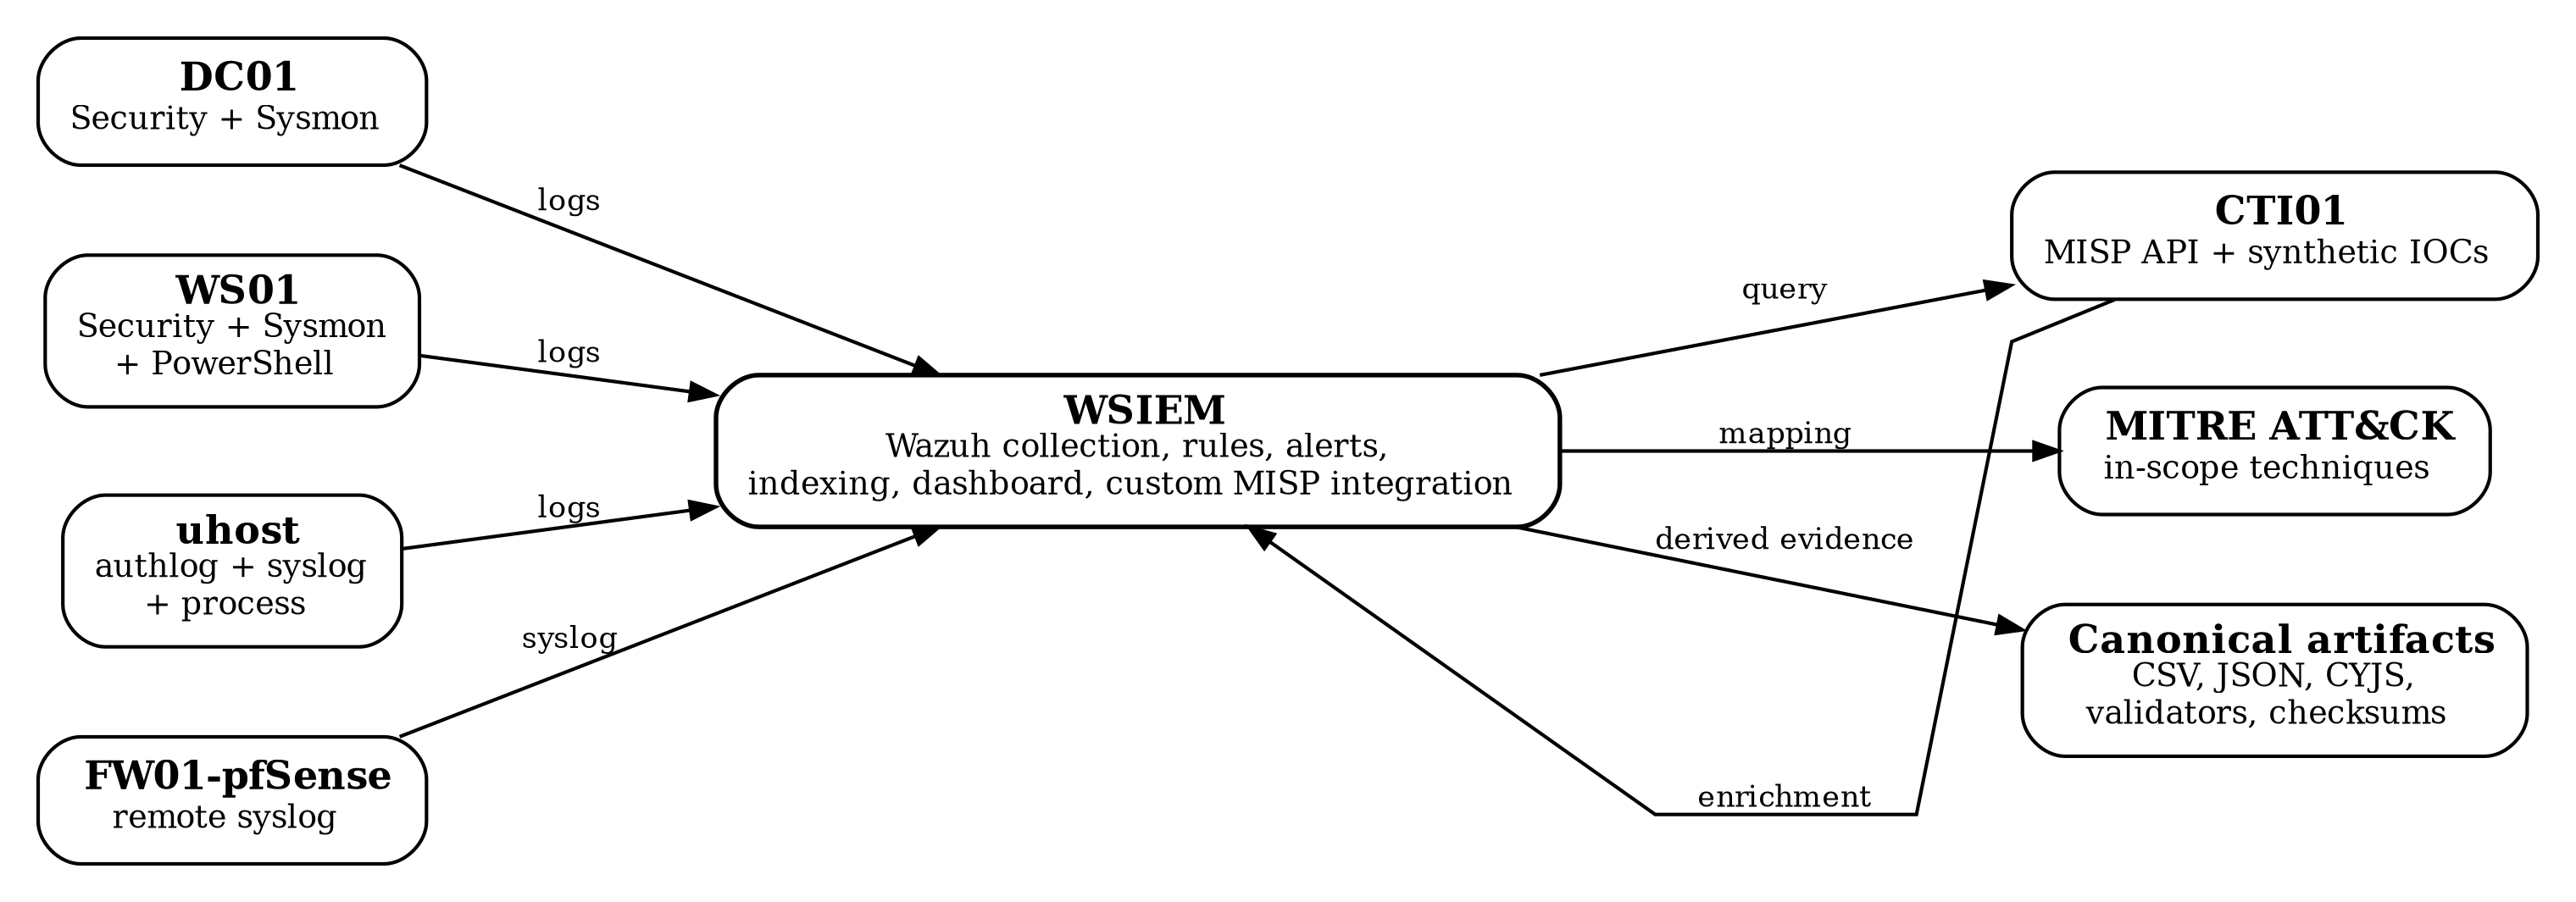
\includegraphics[width=0.92\textwidth]{figures/saci_topology.png}
\caption{Controlled six-asset Wazuh-MISP laboratory and the principal evidence paths used by SACI.}
\label{fig:topology}
\end{figure*}

\begin{table*}[!t]
\caption{Controlled Laboratory Assets and Declared Telemetry Sources}
\label{tab:assets}
\centering
\small
\begin{tabularx}{\textwidth}{p{1.5cm} p{2.5cm} p{2.7cm} Y Y}
\toprule
\textbf{Asset} & \textbf{Logical role} & \textbf{Address} & \textbf{Expected evidence} & \textbf{Primary function in SACI} \\
\midrule
A01 DC01 & Windows domain controller & 192.168.1.10 & Security; Sysmon & Critical identity and endpoint telemetry; controlled Windows scenarios \\
A02 WSIEM & Central SIEM & 192.168.1.100 & ossec; MISP enrichment & Wazuh collection, rules, alerts, custom integration, score inputs \\
A03 CTI01 & CTI platform & 192.168.1.101 & MISP API & IOC storage, query, match, and enrichment response \\
A04 WS01 & Windows workstation & 192.168.1.111 & Security; Sysmon; PowerShell & Endpoint, process, and script visibility \\
A05 uhost & Ubuntu host & 192.168.1.121 & authlog; syslog; process & Linux authentication, system, and process evidence \\
A07 FW01-PFSENSE & Network firewall & 192.168.1.1 & pfSense syslog & Network and firewall event evidence \\
\bottomrule
\end{tabularx}
\end{table*}

DC01 and WS01 provide Windows Security, Sysmon, and PowerShell event channels. Wazuh can collect Windows \texttt{eventchannel} sources \cite{wazuh_logcollection}; Sysmon adds process, network, and DNS telemetry beyond standard Security auditing \cite{sysmon}, and PowerShell logging exposes script and command content \cite{powershell_logging}. Windows advanced audit policy supports granular security-event generation \cite{windows_audit}. The Ubuntu host contributes authentication, system, and process evidence through conventional journald/rsyslog paths \cite{systemd_journal,rsyslog}. The firewall contributes remote pfSense syslog; Netgate documents the transport configuration and the security limitations of unprotected UDP logging \cite{pfsense_remote}.

Wazuh agents and enrollment are the expected endpoint-to-manager mechanism \cite{wazuh_agent_install,wazuh_enrollment}. Custom rules and decoders bind selected behaviors to control and ATT\&CK metadata \cite{wazuh_customrules,wazuh_mitre}. The final evaluation universe contains six assets, twelve expected asset-log-source pairs, twenty-seven control rows of which twenty-five are enabled, thirteen in-scope ATT\&CK techniques, and two synthetic IOC records.

\subsection{CTI Workflow}
CTI01 exposes the MISP API and two synthetic IOCs. MISP is designed for collaborative storage and operational sharing of indicators and related context \cite{wagner2016,misp_docs,misp_install}. The Wazuh external integration invokes a custom connector, the connector queries MISP, a matching IOC is associated with an alert, and the result is linked to ATT\&CK context \cite{wazuh_integrator,oasis_stix,oasis_taxii}. The published chain distinguishes four stages: expected lookup, MISP match, Wazuh alert conversion, and technique association.

The current CTIC implementation is intentionally reported with a limitation: a configured expectation is used to initialize the lookup stage, and the original connector did not persist a complete request-response-no-hit record for every query. Consequently, CTIC=100 proves closure under the implemented dataset schema, not independent execution of every HTTP transaction. A production design should persist a run identifier, request identifier, indicator, request and response timestamps, status, hit/no-hit result, matched attribute identifier, source-alert identifier, generated-alert identifier, and mapping basis.

\subsection{Scenario Orchestration and Evidence Collection}
The published Windows runner uses Ansible and WinRM to execute benign discovery, DNS, and transfer behaviors against DC01. Ansible documents the authentication and transport requirements for Windows remote management \cite{ansible_winrm}. The runner records scenario, command, expected rule, expected ATT\&CK technique, timestamps, and return codes in JSONL, waits for Wazuh ingestion, and inspects the alert stream for selected rule identifiers. JSON and CSV publication formats follow common machine-readable conventions \cite{rfc8259,rfc4180}.

Linux, pfSense, and CTI outcome evidence is included in the canonical coverage and graph files; equivalent end-to-end provisioning and behavior-generation scripts were not preserved for all paths. This difference is explicit: the study audits a verified evidence snapshot and a partial reconstruction scaffold, not a perfect replay of every original host action.

\subsection{Scoring, Graph Generation, and Packaging}
The scorer normalizes Wazuh alerts, MISP enrichment records, scenario events, pfSense events, scope inventories, control definitions, technique scope, IOC expectations, and weights into coverage tables. The graph generator derives node and edge files, CYJS, and Mermaid from those tables. ATT\&CK identifiers can be checked against MITRE's STIX and TAXII data services \cite{mitre_tools,oasis_stix,oasis_taxii}. The portal uses Cytoscape.js for interactive inspection and Mermaid for a version-controlled textual representation \cite{cytoscapejs,mermaid}.

Release order is significant. Coverage and graph artifacts are written first, integrity results second, manifest metadata third, the canonical archive fourth, and the SHA-256 ledger last. The manifest does not recursively hash itself or an archive that embeds the manifest. The canonical archive contains twenty-four files and includes \path{SHA256SUMS.txt}; SHA-256 follows FIPS 180-4 \cite{fips1804}. The read-only \texttt{--check} mode verifies integrity without rewriting \path{integrity_summary.json}, allowing two consecutive validations to produce stable hashes.

\subsection{Reproduction Scaffold}
The repository includes a Vagrantfile, \path{lab/topology.json}, provisioning helpers, and validation scripts. The \texttt{evidence} profile starts a minimal WSIEM role and validates canonical artifacts. The \texttt{portable} profile uses Linux substitutes for topology testing. The \texttt{native} profile expects compatible Windows or FreeBSD boxes and provider configuration. Network mode, optional service deployment, and provider-specific access values are externalized as environment variables; secrets are not embedded in the repository. Vagrant and its VMware provider define the relevant abstraction and provider interfaces \cite{vagrant_docs,vagrant_vmware}.

This scaffold supports artifact recomputation and topology reconstruction at different assurance levels. It is not an exact digital twin because the release does not preserve all original product versions, private boxes, credentials, Sysmon XML, PowerShell policies, pfSense transport settings, MISP secrets, or raw live-log snapshots. This boundary follows reproducibility guidance that distinguishes repeatable computational artifacts from independent replication of an experimental environment \cite{nas_repro,acm_artifacts}.

\section{Results}
\subsection{Canonical Coverage Result}
Table~\ref{tab:finalscores} reports the canonical final snapshot. All twelve expected asset-log pairs were observed. Controls C003 and C004 are documented disabled legacy controls; all twenty-five enabled controls were seen. All thirteen selected techniques have \texttt{covered=1}. Each of two IOC records closes all four CTI flags. The newest global event was in the first freshness tier. All five components and SACI therefore equal 100.

\begin{table}[!t]
\caption{Canonical SACI Coverage Result}
\label{tab:finalscores}
\centering
\small
\begin{tabular}{lrrr}
\toprule
\textbf{Metric} & \textbf{Weight} & \textbf{Closure} & \textbf{Score} \\
\midrule
CWLC & 0.30 & 12/12 pairs & 100.00 \\
CAC & 0.25 & 25/25 controls & 100.00 \\
MDC & 0.20 & 13/13 techniques & 100.00 \\
CTIC & 0.15 & 8/8 flags & 100.00 \\
TF & 0.10 & $\Delta\leq60$ min & 100.00 \\
\midrule
SACI & 1.00 & active weights & 100.00 \\
\bottomrule
\end{tabular}
\end{table}

SACI=100 records complete closure of the declared component expectations under the implemented schema. Broader claims about field detection effectiveness and inventory completeness are evaluated separately under threats to validity.

\subsection{Pre-release Integrity Case F-01}
F-01 is reported as a pre-release validation case, not as a theoretical discovery. After the numerical result had reached 100, the first publication snapshot still contained a mismatch: 171/171 relationship rows were marked observed, while the renderer produced ninety-nine nodes from only ninety-seven declarations. The implicit endpoints were \texttt{LOGSOURCE:Wazuh} and \texttt{MITRE:T1071.001}. Six source--relationship--target triples lacked distinct evidence identifiers, six isolated nodes lacked policy justification, and rule 110203 carried incompatible direct-mapping semantics across the control and CTI tables. The case exposed a defect in the artifact-generation process and supplied a concrete regression target for the independent gate.

\begin{figure*}[!t]
\centering
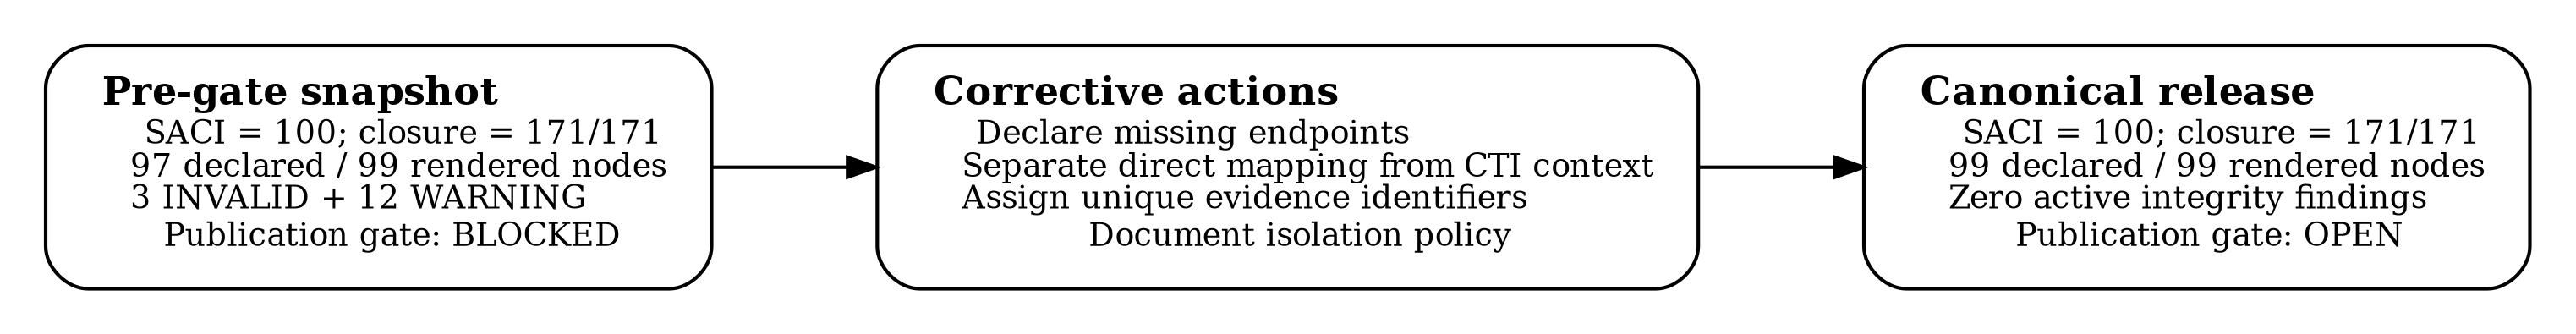
\includegraphics[width=0.94\textwidth]{figures/integrity_f01.png}
\caption{Pre-release case F-01: correction of a numerically closed but structurally invalid artifact before canonical publication.}
\label{fig:f01}
\end{figure*}

The initial integrity result was three INVALID findings and twelve WARNING findings, so the publication gate was BLOCKED even though SACI was 100. Corrective resolution proceeded as follows. First, both missing endpoints were explicitly declared. Second, the direct rule mapping was fixed as 110203$\rightarrow$T1071.001, while T1071.004 from the MISP chain was modeled as CTI context using \texttt{contextualized\_as}. This distinction follows the requirement for precise, evidence-based ATT\&CK mapping \cite{cisa_mapping}. Third, the six parallel triples were retained but assigned unique \texttt{evidence\_id} and \texttt{evidence\_origin} values. Fourth, the two disabled controls, their legacy rules, one historical technique, and the aggregate SACI metric node were documented as permitted isolation cases.

\begin{table*}[!t]
\caption{Pre-release F-01 Integrity Correction}
\label{tab:f01}
\centering
\small
\begin{tabularx}{\textwidth}{Y C C Y}
\toprule
\textbf{Property} & \textbf{Pre-gate snapshot} & \textbf{Canonical release} & \textbf{Resolution semantics} \\
\midrule
Declared/rendered nodes & 97/99 & 99/99 & Missing endpoints explicitly added to the node inventory \\
Observed relationship rows & 171/171 & 171/171 & Coverage closure unchanged \\
Unique triples & 165 & 165 & Parallel evidence retained rather than silently deduplicated \\
Distinct evidence identifiers & Not required for six repeated triples & 171/171 & Every evidence row has stable identity and origin \\
Rule 110203 semantics & Direct T1071.001 and conflicting T1071.004 & Direct T1071.001; contextual T1071.004 & Mapping basis distinguishes detection logic from CTI context \\
Isolated nodes & Six undocumented & Six policy-documented & Historical, disabled, and aggregate roles made explicit \\
Active findings & 3 INVALID, 12 WARNING & 0 & All mandatory integrity checks pass \\
Publication gate & BLOCKED & OPEN & Fail-closed policy permits only VALID datasets \\
SACI & 100 & 100 & Integrity correction did not alter coverage numerators or denominators \\
\bottomrule
\end{tabularx}
\end{table*}

After correction, the canonical graph contains ninety-nine declared and rendered nodes, 171 observed relationship rows, 165 unique triples, eighteen relationship labels, and zero active findings. The integrity status is VALID and the publication gate is OPEN. The unchanged SACI value demonstrates the intended separation: coverage is calculated from the declared coverage tables, while publication requires an independently valid graph and package.

The F-01 case demonstrates why a score and a publication validator must be independent, but the general evaluation of RQ2 is provided by the controlled fault matrix below rather than by treating this implementation defect as a scientific discovery.

\subsection{Controlled Integrity Fault Injection}
Table~\ref{tab:integrityfaults} reports the preregistered and observed outcomes of the nine-case integrity experiment. Every mutation was classified as expected. Referential, schema, mapping, representation, and evidence-identity contradictions produced INVALID. Removing the policy justification from an intentionally isolated node produced VALID\_WITH\_WARNINGS and therefore kept the publication gate BLOCKED. The valid baseline and the documented isolation case remained VALID.

\begin{table*}[!t]
\caption{Controlled Integrity-Gate Fault Injection Results}
\label{tab:integrityfaults}
\centering
\small
\begin{tabularx}{\textwidth}{p{3.1cm} p{2.2cm} p{2.2cm} Y}
\toprule
\textbf{Case} & \textbf{Expected} & \textbf{Observed} & \textbf{Triggered validation class} \\
\midrule
Valid canonical-cardinality baseline & VALID & VALID & No active finding \\
Undeclared edge endpoint & INVALID & INVALID & Referential integrity \\
Duplicate node identifier & INVALID & INVALID & Node identity \\
Conflicting direct ATT\&CK mapping & INVALID & INVALID & Mapping consistency \\
CSV--renderer edge mismatch & INVALID & INVALID & Representation consistency \\
Missing required edge field & INVALID & INVALID & Schema completeness \\
Parallel evidence-ID collision & INVALID & INVALID & Evidence-row identity \\
Undocumented isolated node & VALID+WARN. & VALID+WARN. & Isolation policy \\
Policy-documented isolated node & VALID & VALID & Approved exception \\
\bottomrule
\end{tabularx}
\end{table*}

The matrix answers RQ2 affirmatively at the implemented rule level: the gate distinguishes numerical closure from multiple classes of structurally invalid or review-required publication artifacts. The experiment demonstrates validator selectivity; it does not imply that every possible semantic error in upstream telemetry can be detected.

\subsection{Synthetic Integrity-Gate Scalability}
The cardinality benchmark in Table~\ref{tab:scalability} preserves the ratio and duplicate-evidence structure of the canonical graph while assigning distinct identifiers to each replica. Median validation time increased from 0.778~ms for 99 nodes and 171 rows to 883.438~ms for 99,000 nodes and 171,000 rows. Median peak traced memory increased from 0.035 to 41.17~MiB. All 28 timed validations returned VALID.

\begin{table}[!t]
\caption{Synthetic Integrity Validation Scalability}
\label{tab:scalability}
\centering
\scriptsize
\begin{tabular}{rrrrr}
\toprule
\textbf{Factor} & \textbf{Nodes} & \textbf{Rows} & \textbf{Median ms} & \textbf{Peak MiB} \\
\midrule
1 & 99 & 171 & 0.778 & 0.035 \\
10 & 990 & 1,710 & 5.763 & 0.308 \\
100 & 9,900 & 17,100 & 67.691 & 4.270 \\
1000 & 99,000 & 171,000 & 883.438 & 41.170 \\
\bottomrule
\end{tabular}
\end{table}

The observed growth is compatible with a near-linear pass over nodes and edges for this implementation and size range. RQ4 is therefore answered for integrity-rule execution under synthetic replication: the largest tested graph remained below one second in the stated environment. This result is not evidence of end-to-end SIEM scalability, concurrent ingestion capacity, or browser visualization performance.

\subsection{Deterministic Score Sensitivity and Fault Injection}
The historical S0--S18 score suite contains twenty conditions under nineteen labels because S7 has critical and noncritical branches. The suite is maintained separately from the canonical final snapshot. It is not a sample of independent real-world incidents and does not support confidence intervals or causal effect estimates. It is a deterministic perturbation suite designed to check direction, weight ordering, and recovery behavior.

\begin{figure*}[!t]
\centering
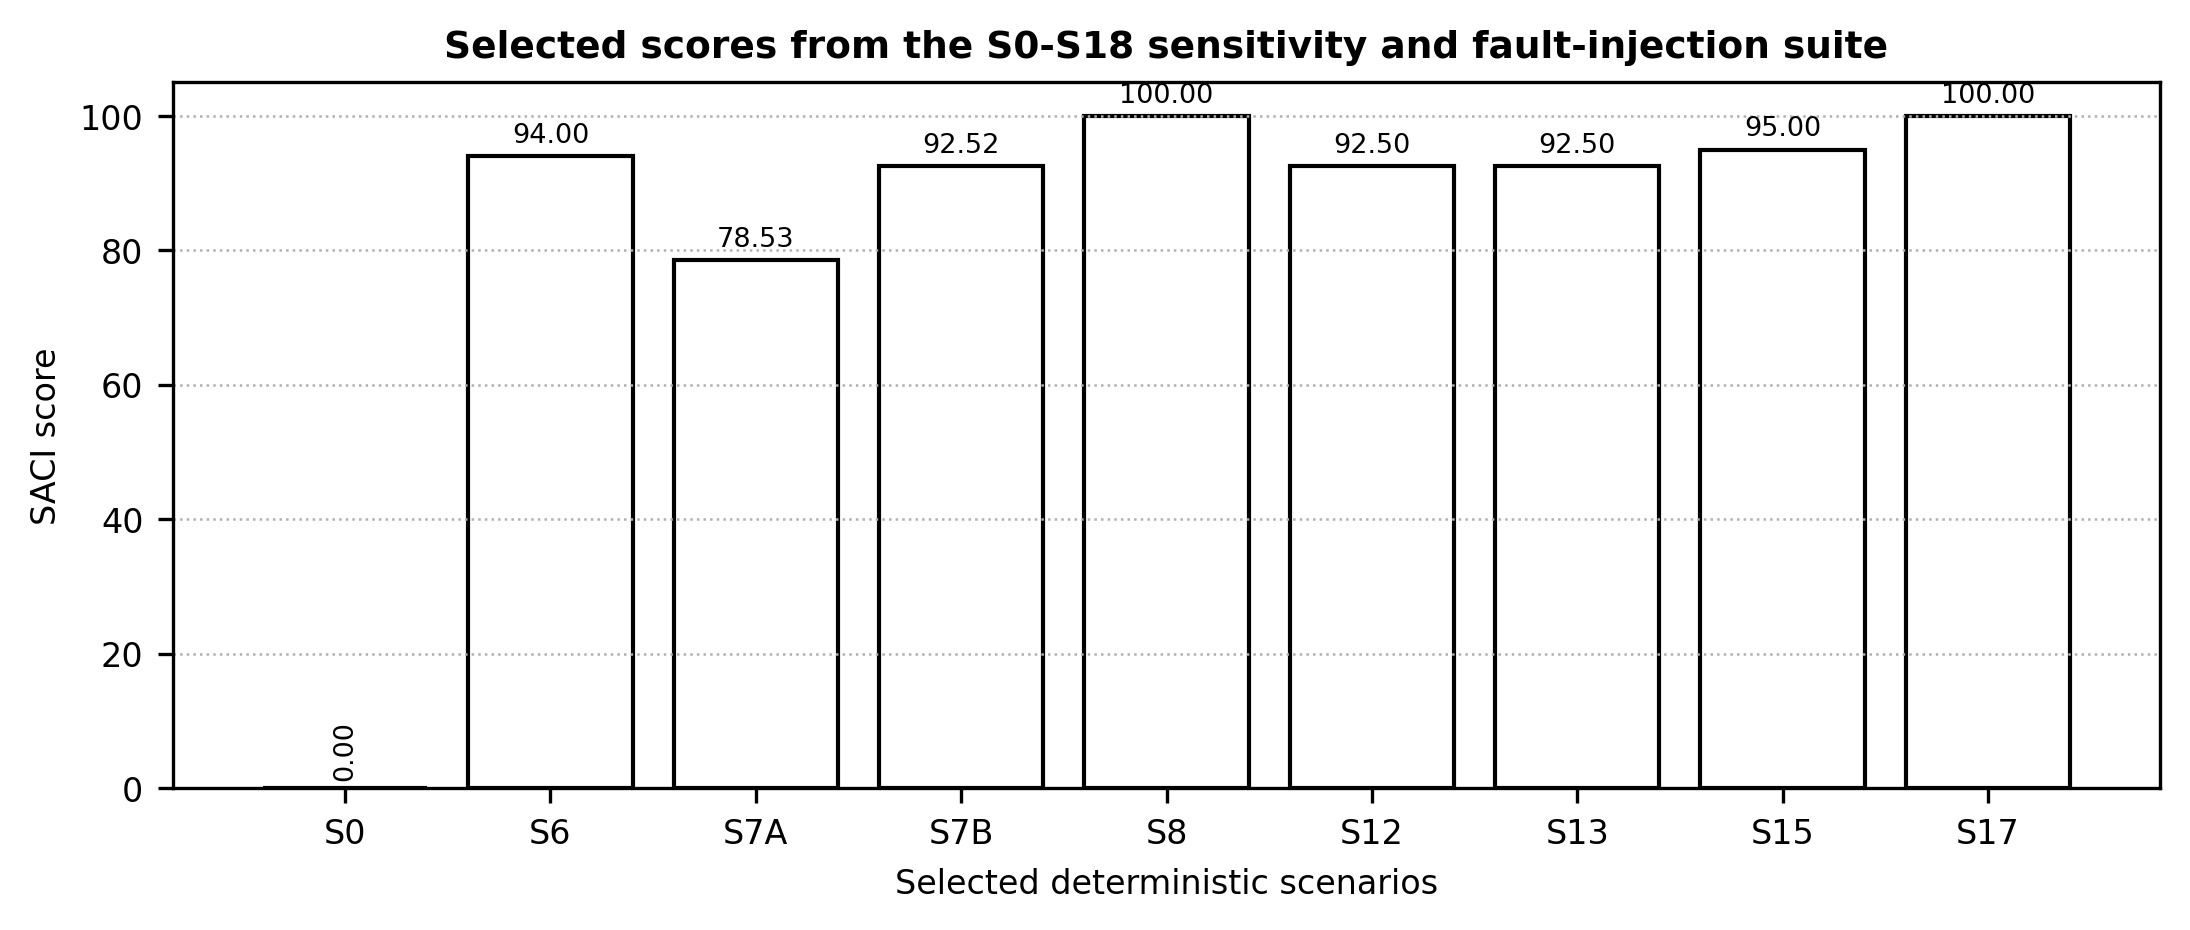
\includegraphics[width=0.93\textwidth]{figures/sensitivity_selected.png}
\caption{Selected scores from the deterministic S0--S18 sensitivity and fault-injection suite. Historical S8 uses a different 95-node/173-edge graph and is not merged with the canonical 99-node/171-edge release.}
\label{fig:sensitivity}
\end{figure*}

Selected results are shown in Fig.~\ref{fig:sensitivity}. SACI rises from 0.00 at S0 to 94.00 after CTI integration at S6 and 100.00 at historical S8 closure. Removing critical DC01 Sysmon evidence produces 78.53 in S7A, whereas the noncritical WS01 loss produces 92.52 in S7B. This difference follows the criticality term in (\ref{eq:cwlc}). CTI perturbations S12 and S13 both produce 92.50 because they remove the same weighted CTIC contribution. Freshness decay in S15 produces 95.00, and S17 recovery returns to 100.00.

These score results answer RQ3 at the level supported by the design: the implementation responds in the expected direction to controlled input changes and applies the declared weight ordering. They do not establish predictive accuracy, field effectiveness, or statistical generalization.

\subsection{Auditability and Hash Stability}
The final release includes coverage tables, score files, node and edge tables, CYJS and Mermaid graphs, reason-code outputs, integrity policy and findings, audit summaries, source code, manifest metadata, and a checksum ledger. The combined validator checks the academic site, canonical dataset, historical-scenario separation, Vagrant syntax, topology metadata, and integrity gate. The full sequence was executed twice consecutively. Both runs produced 99/99 nodes, 171/171 observed rows, no missing relations, zero findings, VALID, OPEN, and unchanged hashes.

This result supports artifact repeatability, not upstream evidence authenticity. A valid checksum proves that a file is unchanged relative to the recorded digest; it does not prove that the original log was generated by the claimed host or that its timestamp was not manipulated. Stronger provenance would require signed collection, immutable run identifiers, raw-event snapshots, synchronized time, and independent custody controls.

\section{Discussion}
\subsection{Answer to RQ1 and Operational Interpretation}
RQ1 is answered affirmatively within the declared laboratory scope. Heterogeneous telemetry and CTI context can be normalized into auditable numerators and denominators, summarized as a component vector and composite score, and linked to provenance graph rows. The final vector $(100,100,100,100,100)$ is directly supported by twelve asset-log pairs, twenty-five enabled controls, thirteen techniques, eight CTI flags, and the freshness tier.

The component vector should always accompany the composite. Two runs with different active metric sets, scopes, control states, technique lists, or weights do not share the same denominator and are not automatically comparable. A documented policy may exclude a disabled legacy control, but an enabled control without evidence must remain a gap. Similarly, criticality is a declared prioritization parameter, not a probability that a host will be attacked.

SACI can support three operational uses: (i) a release or publication gate for a fixed evidence package, (ii) an evidence-completeness audit for a declared environment, and (iii) a longitudinal indicator when scope and policy remain versioned and stable. It should not rank organizations, teams, or SIEM products across heterogeneous scopes without external calibration.

\subsection{Why the Graph Is Supportive Rather Than Scoring}
The graph makes provenance inspectable. A reviewer can traverse an asset to its source, control, rule, ATT\&CK technique, CTI object, integration, and metric contribution. It also allows referential and semantic checks that flat score files do not expose. However, graph centrality, path probability, or attack-graph reachability is not used in the SACI formula. This boundary differentiates SACI from attack graphs and probabilistic risk models and prevents an explanatory representation from being mistaken for an independent validation dataset \cite{manadhata2011,liu2022}.

The F-01 pre-release case illustrates the value of this separation. The score was mathematically complete while the artifact graph was structurally invalid. The independent gate exposed the contradiction and blocked publication without rewriting coverage. The controlled fault matrix then generalized the check beyond that single implementation defect by exercising eight additional structural and policy cases.

\subsection{Threats to Validity}
\textbf{Construct validity:} SACI measures declared evidence closure. It does not measure detection probability, prevention effectiveness, false alarms, mean time to detect, residual risk, adversary success, or business impact. The use of the term ``coverage'' is intentionally bounded to the declared evidence universe.

\textbf{Internal validity:} Some scenario records contain expected rule and technique labels that can survive independently of successful command execution. CTIC's lookup flag is expectation-derived. TF uses the globally newest event. These design choices can overstate closure if upstream execution or attribution is wrong. The integrity gate catches schema and graph contradictions but not every semantic or authenticity error.

\textbf{External validity:} The evaluation uses one six-asset Wazuh--MISP laboratory, two synthetic IOCs, thirteen selected techniques, and a limited set of controlled scenarios. The cardinality benchmark replicates graph structure rather than live telemetry, so it supports only the computational behavior of the integrity checks. Results cannot be generalized to arbitrary enterprise environments, other SIEM products, ingestion throughput, or field detection effectiveness without independent replication.

\textbf{Reproducibility validity:} The artifact package supports arithmetic, graph, manifest, and validator replay. It does not contain all original software versions, secrets, raw logs, provider boxes, or complete end-to-end automation. The Vagrant scaffold is therefore a documented starting point rather than a preserved digital twin.

\textbf{Statistical conclusion validity:} The twenty sensitivity conditions are deterministic tests, not independent samples. No distributional assumptions, repeated randomized trials, confidence intervals, or field outcomes are available. The suite validates implementation direction and recovery behavior, not effect sizes or prediction.

\subsection{Productionization Requirements and Future Work}
The next scoring revision should replace global TF with source-based freshness. Each expected asset-source pair should carry a source timestamp, age, threshold policy, and freshness value; the component should aggregate these values with the same criticality and source weights used in CWLC. This change prevents one fresh stream from masking several stale streams and aligns temporal status with the age-of-information principle \cite{kaul2012}.

CTIC should be rebuilt from actual request-response evidence. Every lookup should persist request and response identifiers, status, hit or no-hit outcome, matched object, source alert, generated alert, and mapping basis. A valid no-hit should not be penalized for lacking alert and mapping stages when those stages are not applicable; an API error or absent response must not be hidden as no-hit or N/A.

Scope completeness should also be measured. The current model assumes the declared asset inventory is the evaluation universe. Production use should report observed-but-undeclared assets and sources, declared-but-never-observed assets, inventory drift, and policy changes. Control lifecycle states should distinguish enabled and applicable, disabled but required, temporarily unavailable, retired with replacement, and not applicable.

Finally, future validation should include independent laboratories, repeated runs, raw-event preservation, other SIEM products, calibrated weight sensitivity, baseline comparisons, negative tests, and preregistered hypotheses. Natural-language explanation should remain downstream of deterministic evidence and should cite the exact rows used to generate each claim.

\section{Data and Artifact Availability}
The canonical source repository, data package, validators, Vagrant scaffold, and portal are publicly available at \url{https://github.com/4rslanismet/saci-final-evidence} and \url{https://4rslanismet.github.io/saci-final-evidence/} \cite{arslan_artifact}. The canonical release is identified by 99 declared and rendered nodes, 171 observed relationship rows, zero active integrity findings, status VALID, and publication gate OPEN. Historical S0--S18 scenarios are stored separately and are not merged with the canonical dataset.

\section{Conclusion}
SACI demonstrates that a declared SIEM--CTI evidence universe can be transformed into an auditable component vector, a simple-additive composite coverage score, a provenance graph, and a fail-closed publication decision. The controlled final snapshot closes all twelve expected asset--source pairs, twenty-five enabled controls, thirteen in-scope ATT\&CK techniques, and eight configured CTI workflow flags, yielding SACI=100.

The principal contribution is the measurement protocol that keeps scope, observation, scoring, provenance, and publication validity separate. Pre-release case F-01 showed how a numerically closed artifact could still contain referential and semantic defects. Rather than treating that software defect as a theoretical discovery, the revised evaluation uses it as a regression case and adds a nine-case controlled integrity matrix. Every injected case produced its expected state, and a synthetic replication benchmark validated 99,000 nodes and 171,000 relationship rows in a median 0.88~s with 41.17~MiB peak traced memory in the stated Python environment.

The result is bounded by the declared scope and evidence schema. Source-based freshness, request--response-derived CTIC, inventory-drift measurement, stronger evidence authenticity, independent laboratories, other SIEM products, and repeated field evaluation remain necessary extensions. By publishing formulas, component tables, graph artifacts, benchmark code, checksums, integrity policy, and the reproduction scaffold together, SACI provides a transparent and falsifiable basis for those extensions.

\newpage
\IEEEtriggeratref{53}
\bibliographystyle{IEEEtran}
\bibliography{saci_idap26}

\end{document}
